%%%%%%%%%%%%%%%%%%%%%%%%%%%%%%%%%%%%%%%%%%%%%%%%%%%%%%%%%%%%%%%%%%%%%%%%%%%%%%%
%%
%%            author(s): Fagner de Assis Moura Pimentel
%%          description: Modelo de trabalho de Conclusão de Curso (TCC)
%
%%                  **  NÂO ALTERAR ESTE ARQUIVO **
%%       No arquivo *info.tex* selecione a fase atual do seu TCC.
%%%%%%%%%%%%%%%%%%%%%%%%%%%%%%%%%%%%%%%%%%%%%%%%%%%%%%%%%%%%%%%%%%%%%%%%%%%%%%%
\documentclass{fei}
\usepackage[colorinlistoftodos,textsize=tiny]{todonotes}
\usepackage{xcolor,colortbl}
\usepackage{lipsum}  
\usepackage{ifthen}
\usepackage{caption}

\addbibresource{referencias.bib}
% Selecione a fase atual do TCC: 
%     TCC 1 -> Projeto
%     TCC 2 -> Trabalho de Conclusão de Curso 
% [ Projeto | Trabalho de Conclusão de Curso ]
\newcommand{\faseAtual}{Trabalho de Conclusão de Curso} 

% Dados do Orientador
\newcommand{\orientador}{Prof. Dr. Fagner de Assis Moura Pimentel}
\newcommand{\departamento}{Ciência da Computação}

% Dados dos Alunos
\newcommand{\alunoCurso} {Ciência da Computação}
\newcommand{\alunoUm}    {Guilherme Reis Queiros de Souza} % Alterar
\newcommand{\alunoDois}  {Gustavo Miranda de Oliveira} % Alterar
\newcommand{\alunoTres}  {Luiz Henrique Silveira} % Alterar
\newcommand{\alunoQuatro}{João Victor da Silva Paula} % Alterar
\newcommand{\alunoCinco} {Vinícius Cristiano Nagatomo de Andrade} % Alterar

% Dados do Projeto
\newcommand{\titulo}{Influência de emoções em jogos} % Alterar
\newcommand{\sub}{ Uso de emoções humanas como variável de entrada em jogos digitais. } % Alterar

% Resumo e palavras chaves
\newcommand{\resumoTrabalho}{
    RESUMO% Alterar
}
\newcommand{\palavraChaveUm}    {Emoções} % Alterar
\newcommand{\palavraChaveDois}  {Jogos Digitais} % Alterar
\newcommand{\palavraChaveTres}  {Inteligência Artificial} % Alterar
\newcommand{\palavraChaveQuatro}{Sinais Neurais} % Alterar
\newcommand{\palavraChaveCinco} {Predição Estatística} % Alterar
\newcommand{\palavraChaveSeis} {Sistemas Sensíveis a Contexto} % Alterar

\newcommand{\source}[1]{\hfill \footnotesize{Fonte: {#1}}}




% \usepackage[utf8]{inputenc}
% \usepackage[table]{xcolor}
% \usepackage{biblatex}

% \usepackage[
%backend=biber,
%style=alphabetic,
%sorting=ynt
%]{biblatex}

% \usepackage{pgfplots}
% \pgfplotsset{compat=1.7}
% \usepackage{pgfplots}
% \usetikzlibrary{calc}
% \usepackage{amsmath}
% \usepackage{subcaption}
% \usepackage[utf8]{inputenc}
% \usepackage{comment}
\usepackage{acronym} 
\usepackage[symbols]{glossaries}

\author{
\alunoUm\\
\alunoDois\\
\alunoTres\\
\alunoQuatro\\
\alunoCinco
}

\title{\titulo}
\subtitulo{\sub}

%%%% -- Entradas Listas de Abreviaturas e Simbolos
%%%%%%%%%%%%%%%%%%%%%%%%%%%%%%%%%%%%%%%%%%%%%%%%%%%%%%%%%%%%%%%%%%%%%%%%%%%%%%%%%%%%%%%%%%%%%%%%%%%%%%%%%
%%%% -- Titulos - comentar caso a respectiva lista nao seja utilizada
\newglossaryentry{acro}{name={},description={\nopostdesc},sort=a} %Usado para alinhar a lista de abreviaturas
\newglossaryentry{geral}{name={Geral},description={\nopostdesc},sort=a}
\newglossaryentry{greek}{name={Letras gregas},description={\nopostdesc},sort=b}
\newglossaryentry{sub}{name={Subscritos},description={\nopostdesc},sort=c}

%% -- Abreviaturas
\newacronym[longplural=Computational Aided Design,parent=acro]{cad}{CAD}{Computational Aided Design}
\newacronym[longplural=Centro Universitário da FEI,parent=acro]{fei}{FEI}{Centro Universitário da FEI}

%% -- Simbolos
%% -- Latin letters
%\newglossaryentry{}{parent=geral,type=symbols,name={},sort=a,description={}

\newglossaryentry{A}{parent=geral,type=symbols,name={\ensuremath{A}},sort=a,description={exchanger total heat transfer area, $m^2$}}
\newglossaryentry{G}{parent=geral,type=symbols,name={\ensuremath{G}},sort=g,description={exchanger flow-stream mass velocity, $kg/(s m^2)$}}
\newglossaryentry{f}{parent=geral,type=symbols,name={\ensuremath{j}},sort=j,description={friction factor, dimensionless}}

%% -- Greek letters
%\newglossaryentry{}{parent=geral,type=symbols,name={},sort=a,description={}
\newglossaryentry{deltap}{parent=greek,type=symbols,name={\ensuremath{\Delta P}},sort=p,description={pressure drop, $Pa$}}
\newglossaryentry{nu}{parent=greek,type=symbols,name={\ensuremath{\nu}},sort=b,description={specific volume, $m^3/kg$}}
\newglossaryentry{beta}{parent=greek,type=symbols,name={\ensuremath{\beta}},sort=b,description={ratio of free-flow area $A_{ff}$ and frontal area $A_{fr}$ of one side of exchanger, dimensionless}}

%% -- Subscripts
%\newglossaryentry{}{parent=geral,type=symbols,name={},sort=a,description={}
\newglossaryentry{fr}{parent=sub,type=symbols,name={\ensuremath{fr}},sort=fr,description={frontal}}
\newglossaryentry{in}{parent=sub,type=symbols,name={\ensuremath{i}},sort=in,description={inlet}}
\newglossaryentry{out}{parent=sub,type=symbols,name={\ensuremath{o}},sort=out,description={outlet}}
%%%%%%%%%%%%%%%%%%%%%%%%%%%%%%%%%%%%%%%%%%%%%%%%%%%%%%%%%%%%%%%%%%%%%%%%%%%


\makeindex
\makeglossaries

\begin{document}

\maketitle
\begin{folhaderosto}
    Trabalho de Conclusão de Curso apresentado ao Centro Universitário FEI, como parte dos requisitos necessários para obtenção do título de Bacharel em \alunoCurso. Orientado pelo \orientador.
\end{folhaderosto}

\tableofcontents

% if
\ifthenelse{\equal{\faseAtual}{Projeto}}
% then
{

    % Não alterar esse arquivo
\label{resumo}
\begin{resumo}
%\resumoTrabalho

%\Contexto e objetivo

Emoções são uma das principais características que nos tornam humanos. Algo abstrato, deduzido e catalogado por nós mesmos, que dita toda manifestação da percepção humana no mundo. Um dos grandes desafios atuais da ciência é conseguir, apropriadamente, interceptar e interpretar de forma coesa esses sinais neurais que constituem as emoções. Contudo, após este desafio ser alcançado, o próximo seria como e onde usar essas novas possíveis entradas e variáveis dentro de sistemas digitais. Tendo isso em vista, foi realizado nesse trabalho a interpretação de sinais neurológicos pré-classificados em um sistema de aprendizado de máquina executado ao mesmo tempo que um jogo de computador, sendo este jogo um utilizador da saída destes dados para variar o contexto em que o jogador se encontra, através de um loop de feedback entre o jogador e o jogo. Os métodos utilizados neste trabalho são formados pela interpretação de sinais neurais através de inteligência artificial e detecção de padrões, desenvolvendo novas e melhorando as já existentes metodologias, estratégias e formas de imersão e retenção de público utilizadas na industria de entretenimento voltada para jogos digitais. Também foi utilizado predição de escolhas e emoções através de dados estatísticos de jogabilidades e decisões preexistentes\todo{rever ao desenrolar do projeto}. A proveniência dos sinais neurais se da pelo uso de bases de dados públicas que contemplam detalhes de atividade cerebral de voluntários enquanto tarefas específicas eram desenvolvidas, capturados através de EEG (eletroencefalografia) e outros métodos. Estes e outros métodos e materiais são mais detalhadamente descritos nas próximas sessões deste trabalho.

\palavraschave{\palavraChaveUm; \palavraChaveDois; \palavraChaveTres;  \palavraChaveQuatro; \palavraChaveCinco; \palavraChaveSeis}
\end{resumo}
    \chapter{INTRODUÇÃO}
\label{intro}

Não é de hoje que um dos principais fatores para o avanço da neurociência foram os métodos de detecção de ondas cerebrais \cite{eegimportanciasite}. Através deles, se tornou confiável capturar e interpretar sinais neurais em animais e humanos. No que tange o emocional, diversos estudos foram e ainda são realizados para que dados obtidos por métodos como Eletroencefalograma sejam interpretados de maneira fidedigna.

Neste trabalho, esses dados foram utilizados em um plano de fundo que nos ajude a entender as possibilidades de interação entre a saída desses sinais e um sistema computacional. Este plano de fundo, como destacado, será um jogo de computador que reage aos estados emocionais do jogador dentro de seu ecossistema através de um banco de dados já recolhido para a análise desses sinais.

\section{Contextualização}

A área de pesquisa de captação neural para interpretação desses dados evoluiu muito desde o surgimento de técnicas como o Eletroencefalograma \cite{rocha2022analise}. A partir destes métodos, foram desenvolvidas e maturadas diversas técnicas para que esses dados fossem interpretados em sua completude. Isto é, o que a principio era utilizado apenas para saber níveis de estresse ou relaxamento, devido o conhecimento ainda muito vago na interpretação dos sinais, hoje é utilizado em estudos até mesmo na reconstrução de imagens conjuradas na imaginação \cite{shimizu2022improving}. Para captar estes sinais, métodos como Eletroencefalograma (EEG) podem ser utilizados \cite{moises2020reconhecimento}, bem como outros menos sofisticados, como captação de sinais de ansiedade e estresse para classificar emoções positivas e negativas \cite{nalepa2019emotionalcontext}. Independente dos métodos utilizados, este trabalho transcorre utilizando bases de dados prontas e classificadas como forma de treinamento e entrada num sistema de classificação de padrões. Esse sistema irá, então, se comunicar através de uma interface com um jogo, afim de demonstrar a efetividade e desempenho do algoritmo de interpretação, bem como os impactos de um sistema como esse na jogabilidade e imersão do jogador.

Por sua vez, a área dos jogos digitais é bastante ampla na aplicação de conceitos de programação, inteligência artificial e arte. A maior parte dos jogos incluem em suas experiências algum nível de adaptabilidade com foco no jogador: seletores de dificuldade, filtros de cor para pessoas com daltonismo e até mesmo compatibilidade com controles especiais. Essa capacidade de adaptação tem por finalidade tornar a experiência do usuário mais confortável, mesmo se o jogador tiver algum tipo de deficiência. Esse tipo de adaptabilidade é também chamado de acessibilidade \cite{acessibilidadenosjogos}. 

Contudo, também existe a adaptabilidade que visa não o conforto do jogador, mas a capacidade do jogo de se adaptar a certas formas de interação e responder de formas diferentes a essas interações, gerando experiências diferentes. Essa é uma prática de mais complexa implementação, mas que ganha espaço devido a alta variação na experiência individual de cada jogador e a quantidade maior de possibilidades e caminhos que podem ser percorridos durante uma dessas experiências. Isso traz diferentes experiências para diferentes jogadores, tornando-as mais únicas a cada ambiente e situação.

No entanto, há poucos exemplos no mercado que chegaram ao ponto de capturar diretamente o que um jogador sente para então influenciar a jogabilidade em um loop de feedback: muitos jogos de terror usam o microfone, por exemplo, para monitorar gritos ou falas afim de atrair um monstro. O jogo Emovere \cite{filipa2019emovere} utiliza batimentos cardíacos para influenciar a mecânica de combate. O objetivo deste trabalho é construir um jogo mais próximo do segundo exemplo, utilizando sinais emocionais do jogador para influenciar o ambiente e mecânicas.

\section{Objetivo}

O objetivo deste trabalho é analisar, identificar e classificar determinados sinais neurais que caracterizem estados emocionais, afim de utilizá-los em um sistema final com ênfase na área de jogos digitais utilizando duas bases de dados publicas e outras bases dos trabalhos estudados mais a frente. Com isso, foram estudados os potenciais benefícios e malefícios da influência deste sistema dinâmico em relação a um jogo que não tenha esse sistema, analisando o quanto o jogador é influenciado e o quanto essas mudanças podem agregar a favor ou em detrimento do jogo.

\section{Estrutura do Trabalho}

O restante deste trabalho é dividido da seguinte maneira: No capítulo \ref{conceitos}, são apresentados os principais conceitos que serão utilizados, como Sistemas Sensíveis a Contexto, Emoções por Nível de Excitação e Valência, Loop de Biofeedback, Game Engine e outros. No capítulo \ref{trabs}, são apresentados os principais trabalhos relacionados pesquisados ao longo da elaboração deste trabalho, que é detalhado melhor no capítulo \ref{metodologia}, onde são apresentadas as ferramentas, métodos, materiais e métricas utilizadas para o estudo e elaboração do projeto, como a elaboração do algorítimo de padrões, simulação dentro do jogo construído, treinamento utilizando a base, verificação da eficiência do algorítimo, etc. \todo{completar com o restante dos capitulos}


    \chapter{CONCEITOS FUNDAMENTAIS} \label{conceitos}

Neste capitulo serão abordados todos os conceitos utilizados na realização deste trabalho, como Jogos Digitais, ferramentas para desenvolvimento destes jogos, sistemas sensíveis a contexto, o que são sinais neurais, loop de biofeedback etc. \todo{completar este capitulo com todos os principais conceitos utilizados ao desenrolar do projeto. aprendizado de máquina, métricas de avaliação, base de dados}

\section{Jogos Digitais}
Jogos digitais são aplicações interativas utilizadas como entretenimento. Esses jogos podem ser apresentados em diversas mídias: desde os conhecidos fliperamas e consoles de mesa \cite{batista2018estudo}, até os jogados em computadores e smartphones nos dias de hoje. No contexto deste trabalho, foram considerados apenas os jogos de computador como uma plataforma de testes para o algoritmo de interpretação de sinais/emoções.

\section{Game Engine}
Game engine, também conhecido como Motor Gráfico, é um framework de criação de jogos. Esses frameworks são utilizados para facilitar a criação de jogos eletrônicos, já que sua maioria possuem ferramentas agregadas a códigos já prontos de gráficos 2D/3D, simulação de física, desenvolvimento multi-plataforma, comandos I/O, sons e outros sistemas e módulos que, sem o uso de um framework, precisariam ser implementados um a um, poupando muito tempo de desenvolvimento \cite{gameengine}. Grandes desenvolvedoras costumam construir suas próprias Game Engines, mas essas costumam não ser disponibilizadas para o público geral. Para isso, também existem Game Engines públicas, como a Unity \cite{Unitysite}, que é gratuita e utilizada por milhares de usuários no mundo todo para criação de jogos, sendo a escolhida para a realização deste trabalho.

\subsection{Game Engine - Unity}
A plataforma Unity é uma ferramenta de desenvolvimento de jogos 2D e 3D baseada em C\# e estrutura de programação baseada em scripts, oferecendo diversos recursos para facilitação do trabalho de desenvolvedores desse tipo de projeto. Ela é um suporte para todos os recursos necessário no desenvolvimento de jogos digitais, como gráficos, áudio, controles e compatibilidade com diversos dispositivos.
A escolha da Unity se dá pela facilidade de encontrar elementos e projetos para se ter como base, por ser uma engine popular e gratuita, bem como pela experiência já adquirida por sua utilização no decorrer do curso.

\section{Sinais Neurais}
Sinais Neurais são pequenos impulsos nervosos realizados pelas células neurais individuais, sinais esses que são inicialmente transmitidos de maneira elétrica e passam por um processo de conversão para se tornarem químicos. Através de sistemas como o (EEG), ou Eletroencefalograma, podemos registrar os sinais emitidos assim como suas mudanças nas atividades cerebrais durante a execução de diferentes tarefas como pensar, se comunicar ou pegar um objeto, sendo possível a retirada de informações como a analise e interpretação desses impulsos nervosos e seus padrões nas atividades cerebrais, podendo assim ser realizada a investigação de deficiências neurais, estados mentais, sono e comunicação do individuo \cite{rocha2022analise}.

\begin{figure}[h]
    \centering
    \caption{Estrutura de uma célula neuronal realizando uma atividade sináptica.}
    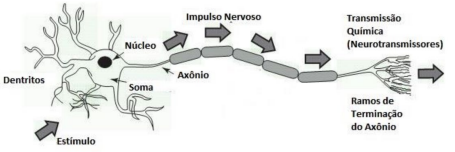
\includegraphics[width=12cm]{Figuras/celula-neural.png}
    \caption*{Fonte: \cite{rocha2022analise}}
    \label{fig:celula_neural}
\end{figure}

\section{Sistemas Sensíveis a Contexto}
Sistemas Sensíveis a Contexto são sistemas que utilizam de pistas contextuais para adaptar-se a alguma necessidade de elementos em seu ambiente. Essas pistas contextuais podem ser dados de ambiente, variáveis dinâmicas que mudam ao executar do programa ou qualquer tipo de informação que seja útil para definir características e comportamentos num cenário \cite{vieira2009modelos}. No âmbito deste projeto, o contexto ao qual o sistema será sensível é a externalização emocional do jogador, que influenciará como o próprio jogo age e reage em seu ambiente.

\section{Loop de biofeedback}
No contexto de medicina, para citar o trabalho do Dr. Michael G. McKEE na área de terapia, 
\textit{"O biofeedback envolve o monitoramento e uso de informações fisiológicas para ensinar os pacientes a modificar funções fisiológicas específicas"}\cite{biofeedback2008biofeedback}. No contexto do nosso projeto, o biofeedback participa de um círculo de interpretação e comportamento. Através dos sinais do jogador, o jogo irá adaptar-se e mudar o modo com que interage com o jogador. Com isso, o jogador tem a oportunidade de tentar controlar esses sinais afim de aproveitar melhor de um aspecto ou outro de uma mecânica. 

\section{Computação Afetiva}
Com o uso massivo de bases de dados e experimentos com o uso de inteligencias artificiais para uma interação mais humana. O termo Computação Afetiva explora justamente o comportamento das interações Humano-computador, ou seja, o modo como as maquinas podem reconhecer, interpretar e influenciar um sentimento humano. Em relação a área de jogos, o artigo \cite{filipa2019emovere} mostra a possibilidade de criar o desenvolvimento de estratégias afim de experiencias mais envolventes e personalizadas para cada jogador, onde o jogo responda ao estado emocional atual do jogador, adaptando historia, recompensas e mecânicas para determinada parte do jogo, deixando a experiência mais imersiva e satisfatória.

\break
\section{Emoções por Nível de Excitação e Valência}

 \begin{figure}[h]
    \centering
    \caption{Diagrama de Emoção por nível de Excitação e Valência}
    \centering
    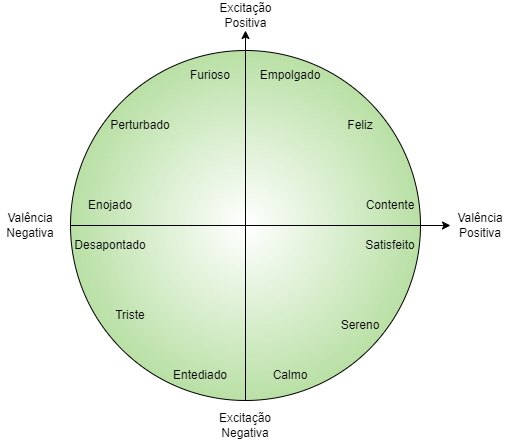
\includegraphics[width=0.5\textwidth]{Figuras/diagrama-emocional.drawio.png}
    \caption*{Fonte: Autores}
    \label{fig:diagrama_emocional}
\end{figure}

Utilizando aparelhos de medição de atividade tanto neurológica quanto fisiológica, é possível medir o nível de estresse, nervosismo ou ansiedade de uma pessoa. Cruzando esses dados com os obtidos através de uma entrevista de feedback, é possível dizer em qual direção estava apontado seu vetor emocional dentro do diagrama de excitação-valência.


    \chapter{Trabalhos Relacionados} \label{trabs}

Tendo em vista como propósito principal deste estudo a classificação em emoções de determinados sinais neurológicos e sua utilização no contexto de jogos digitais, os trabalhos \cite{nalepa2019emotionalcontext} e \cite{filipa2019emovere} foram definidos como principais modelos de estudo.

No trabalho \cite{nalepa2019emotionalcontext}, há a exploração de sistemas capazes de detectar e interpretar os sinais capturados através de equipamentos sensoriais. Foram utilizados nesse trabalho equipamentos de medição sensorial, como o kit BITalino (r)evolution \cite{bitalinoprosuto}, plataforma com diversos sensores de bio-sinais pré-montada, a Pulseira Empatica E4 \cite{empatica4site}, que é um monitor de atividade vestível, capaz de medir diversos dados fisiológicos com precisão, e outros equipamentos para efeito de comparação, como a Microsoft Band 2 \cite{Microsoftband2}, atualmente descontinuado.

Além destes materiais, foram utilizados frameworks para construção de aplicativos de teste, como o AWARE \cite{awaresite}, que é uma plataforma e plugin Android para captura de dados sensoriais, o HeaRTDroid \cite{heartdroidsite}, uma ferramenta para captura de informação contextual dinâmica e interpretação desses dados em meio a ruídos e incertezas, o BandReader \cite{bandreader}, um software que se comunica através de bluetooth com múltiplos dispositivos de aquisição de dados, bem como foram construídos protótipos de jogos afetivos feitos nas game engines Unity e GameMaker.

Para construir o ambiente de teste que, neste caso, é o jogo, foram seguidas técnicas de e Game Design Patterns, que visam definir relações e interações entre diferentes conceitos e elementos dentro de um jogo.

Este trabalho conclui-se trazendo como resultados a avaliação dos jogadores sobre quais protótipos de jogos geraram maior satisfação no que se diz sobre imersão, mecânicas e ajustes dos níveis e fases: os jogos que utilizaram Loop Afetivo ou que não utilizaram.

No trabalho \cite{filipa2019emovere}, o foco principal foi a utilização de um loop de feedback emocional dentro de uma mecânica de combate no jogo Emovere. Através de um sensor de batimentos cardíacos, o pulso do jogador seria detectado, influenciando na jogabilidade, como demonstrado no diagrama de biofeedback abaixo.

\begin{figure}[h]
    \centering
    \caption{Diagramas de loop de combate e biofeedback.}
    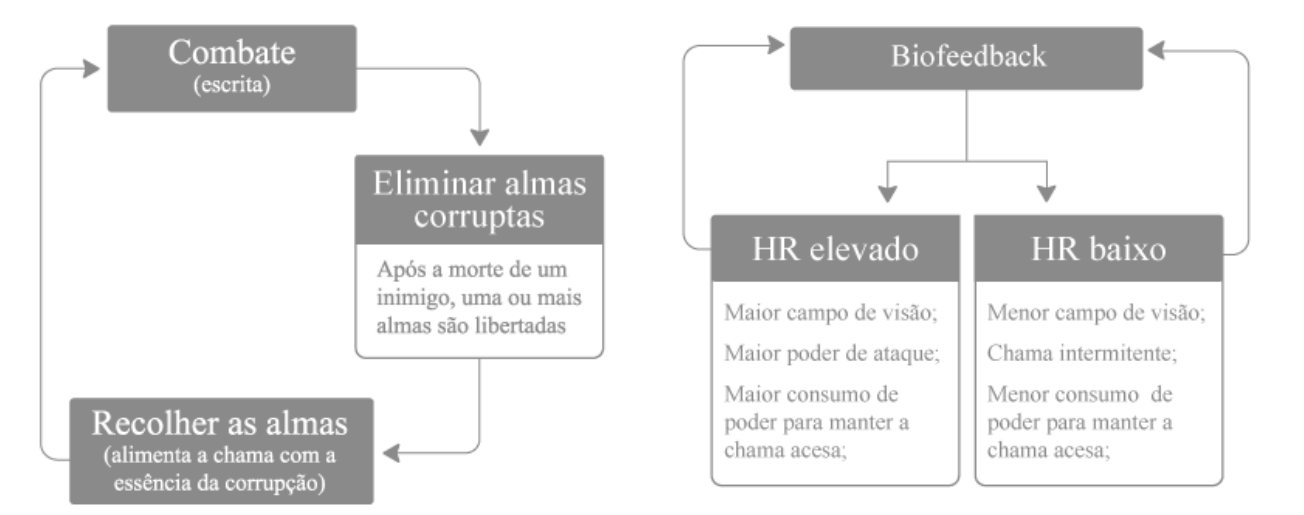
\includegraphics[width=17cm]{Figuras/diagrama-filipa-loop.png}
    \caption*{Fonte: \cite{filipa2019emovere}}
    \label{fig:diagrama_biofeedback}
\end{figure}

Os trabalhos apresentados conseguem cobrir com clareza os aspectos técnicos da implementação, através de métodos e materiais conhecidos e replicáveis. Buscamos aplicar alguns destes conhecimentos neste projeto, sendo eles a game engine Unity e o loop de biofeedback entre jogador e jogo.

Nota-se que grande parte dos recursos e conceitos extraídos e analisados nos trabalhos acima não serão utilizados neste trabalho. Isso se deve ao fato de que, na metodologia que será abordada aqui, não será utilizada detecção em tempo real. Isso está melhor descrito em \ref{metodologia}.

Além destes conteúdos, utilizamos metodologias para leituras de arquivos com dados de sinais neurais e sinais fisiológicos, técnicas de game development e integração de sistemas para agregar o jogo a um sistema de interpretação. Esses processos também estão detalhados em \ref{metodologia} 

Serão focados neste trabalho tentativas para expandir o que foi abordado nos dois projetos mencionados: enquanto ambos trabalham apenas com sinais fisiológicos, serão trabalhados entradas de sinais neurais reconhecidos.
    \chapter{METODOLOGIA}
\label{metodologia}

Será mostrado neste capitulo os materiais, ferramentas e métodos utilizados na realização deste trabalho. Em detalhes, são explicados a constituição e captação dos bancos de sinais neurais, métodos de processamento por injeção de banco de dados no algoritmo, o jogo utilizado como exemplo e as métricas utilizadas para avaliar o trabalho. \todo{listar todo o conteúdo deste capitulo quando o trabalho for finalizado}

\section{Materiais}

\subsection{Banco de Sinais Neurais e Fisiológicos}
Para esse trabalho utilizamos dados que contemplem, de alguma forma, o estado emocional de pessoas dentro de um contexto. Esses dados podem ser encontrados, nas metodologias investigadas na forma de sinais eletromagnéticos "crus" vindo de regiões conhecidas e pré estabelecidas do cérebro.

Uma das formas menos invasivas e melhor desenvolvidas para captação desses sinais é o Eletroencefalograma (EEG). Esse método consiste na utilização de eletrodos para captação de pulsos eletro-magnéticos do cérebro em determinadas regiões que, a depender do tipo de estimulo e feedback verbal do estado emocional reportado por um participante no momento da coleta, serão classificados como positivos ou negativos.

No caso deste trabalho, foram utilizados os bancos \cite{linkbase1} e \cite{linkbase2} que contem dados captados das formas mencionadas para treinar um algoritmo de reconhecimento de padrões. \todo{detalhar melhor os pormenores dos bancos}

\section{Métodos}

% Foram pensadas em duas metodologias levemente distintas em relação a captação dos dados e em como serão utilizados.

% \subsection{Detecção e Feedback Simultâneos}
% A primeira, chamado "Método com detecção e feedback simultâneos" parte do principio que a detecção dos dados, ou seja, a captação dos sinais neurais, ocorrerá ao mesmo tempo que a interpretação e utilização desses dados dentro do jogo. Este é um cenário ideal onde o loop de feedback é fluidamente realizado: o jogador, ao jogar o jogo, gera sinais que, ao serem interpretados pelo algoritmo fazem com que o jogo se adapte passivamente a esses sinais. Com isso, o jogador reage a essa adaptação, gerando um novo fluxo de sinais, e assim sucessivamente. Essa metodologia, além de depender de todos os equipamentos e programas para captação e interpretação correta de sinais, é também um grande desafio de performance e paralelismo.

% \begin{figure}[h]
%     \centering
%     \caption{Diagrama de Metodologia Paralela}
%     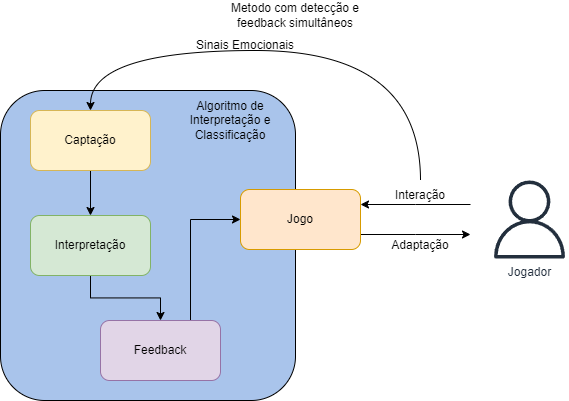
\includegraphics[width=10cm]{Figuras/diagrama-metodologia-um.drawio.png}
%     \caption*{Fonte: Autores}
%     \label{fig:diagrama_metodologia}
% \end{figure}

\subsection{Injeção de Banco de Dados}
Este método é levemente simplificado no setor de pré-interpretação com relação a uma leitura ao-vivo utilizando equipamentos de sensores EEG. Ao invés de ser utilizada a captação ao mesmo tempo que a interpretação dos dados, foi utilizado um banco de dados já classificado e conhecido. Esses dados foram injetados em um algoritmo treinado para sua interpretação e imediata utilização pelo jogo. Dessa forma, ao invés de estarmos testando a verdadeira saída emocional do jogador, focamos na capacidade do algoritmo de interpretação e do jogo de agirem ao mesmo tempo através da injeção dos dados de uma base conhecida no algoritmo. \todo{detalhar melhor o que tem na base de dados}

\begin{figure}[h]
    \centering
    \caption{Diagrama de Metodologia Classificada}
    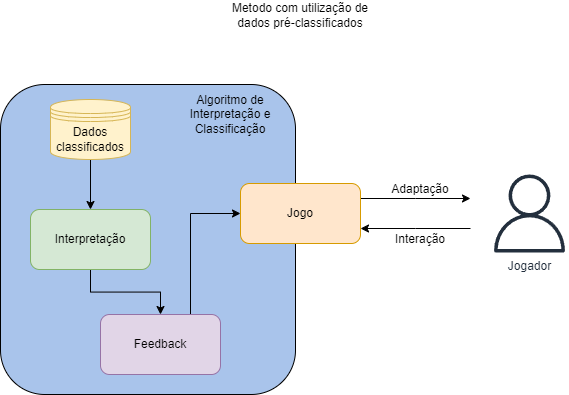
\includegraphics[width=10cm]{Figuras/diagrama-metodologia-dois.drawio.png}
    \caption*{Fonte: Autores}
    \label{fig:diagrama_metodologia}
\end{figure}

Foi optado por essa metodologia por conta da necessidade de permissões para utilizar um método que realizasse a leitura através de equipamentos de EEG durante a execução do jogo em voluntários, mas também para que o foco do trabalho seja a adaptabilidade de um sistema - nesse caso, o jogo - quando utilizada essa entrada de dados. \todo{rever a parte sobre o foco deste trabalho, a depender do desenrolar do projeto}

\subsection{Jogo}
O jogo que utilizamos como base é uma versão modificada dos projetos realizados durante as aulas de Desenvolvimento de Jogos Digitais no sétimo ciclo do curso. Se trata de um jogo de plataforma no estilo de clássicos como \textit{Castlevania} \cite{castlevania} e \textit{Super Metroid} \cite{supermetroid}, melhor detalhado a frente.

\todo{descrição do jogo do projeto. não é versão final.}
No jogo deste projeto, o jogador controla um personagem capaz de se transformar a depender da emoção do jogador. Ao se transformar, as mecânicas do jogo se alteram, mudando como o jogador deve jogar o jogo e as reações do mundo do jogo ao personagem.

O jogo passou por adaptações de compatibilidade com o algoritmo de classificação em tempo real que será desenvolvido, tanto para receber os dados como para implementar as diferentes mecânicas adaptativas.

O jogador pode jogar e testar as novas funcionalidades, por meio de inputs programáveis que serão disponibilizados no jogo. Esses inputs, através de botões, simularão a inserção da emoção do jogador, pois não é permitido captar diretamente as ondas transmitidas pelo usuário.

\section{Métricas}

Como métrica, após o teste das duas diferentes versões do jogo: com sistema de adaptabilidade e sem sistema de adaptabilidade, foi realizado um questionário com perguntas a cerca da satisfação dos jogadores comparando as duas versões. As perguntas giram em torno de três aspectos: 

\begin{itemize}
  \item Satisfação com as Mecânicas: o quanto a mudança de mecânicas agrada com relação as mecânicas padrões não-adaptativas do jogo;
  \item Satisfação com a Imersão: o quanto o jogador se sente mais imerso com relação a imersão sentida na versão não-adaptativa do jogo;
  \item Satisfação Geral: o quanto o jogador gosta mais ou menos do jogo com o sistema adaptativo com relação ao jogo sem o sistema.
\end{itemize}

Essas perguntas foram respondidas em uma escala de -5 a 5, onde -5 é muito menos e +5 é muito mais.

Além disso, foram avaliados o desempenho de algoritmos de leitura de bancos de dados com sinais neurais e fisiológicos, com relação ao tempo de execução, leitura e saída dos dados, para descobrir a viabilidade de sua utilização em simultâneo à execução do jogo. \todo{como será feito?}


    \chapter{Cronograma}
\label{cronograma}

Para organizar o trabalho de forma a seguir um desenvolvimento efetivo, decidiu-se por separar em atividades as principais etapas de desenvolvimento.

\begin{itemize}
    \item \textbf{Atividade 1: Criar o Sistema de Classificação em Tempo Real (SCTR)} Esse sistema será o alicerce do projeto apresentado neste trabalho. Como abordado anteriormente, esse sistema será o responsável por capturar os sinais (ou, neste caso, receber do banco de dados) e imprimi-los em alguma saída ligada a um outro sistema que, neste caso, será o jogo experimental demonstrativo.
    \item \textbf{Atividade 2: Criar o Jogo Experimental} O jogo experimental será desenvolvido em paralelo ao sistema de classificação (que será chamado de SCTR). Dessa forma, será possível realizar ajustes e adaptações de compatibilidade em torno de ambos os programas, facilitando sua integração um ao outro.
    \item \textbf{Atividade 3: Testar o Output do SCTR} Essa etapa focará no tempo de resposta do SCTR. Para que seja possível utilizá-lo em um cenário que exija feedback em tempo real, o tempo de resposta do SCTR deve ser baixo, desde o momento da entrada de dados até o processamento e saída da classificação.
    \item \textbf{Atividade 4: Implementar SCTR ao Jogo} Com o desenvolvimento em paralelo dedicado por mais tempo na Atividade 1, a etapa de implementação e entre esses dois sistemas será breve, focando em possíveis problemas de tempo de resposta e outros pormenores.
    \item \textbf{Atividade 5: Baterias de Testes e Correções} Baterias de testes transcorrerão com uma versão dos programas que seja considerada "final" em um cenário real de produção. Com isso, espera-se a captura de mais erros e suas posteriores correções.
    \item \textbf{Atividade 6: Levantamento de Resultados} Finalmente, serão classificados os resultados, tomando comparativos e métricas de melhora durante o projeto e o que espera-se de ser desempenho e futuro.
\end{itemize}

\begin{table}[h]
\caption{Cronograma de execução do projeto.}
\label{tab:cronograma}
\resizebox{\textwidth}{!}{
\begin{tabular}{|l|c|c|c|c|c|c|c|c|c|c|c|c|}
\hline
Atividade / Mês & 7 & 8 & 9 & 10 & 11 & 12 \\ \hline
Atividade 1 & \gray & \gray & \gray & \gray &  & \\ \hline
Atividade 2 & \gray & \gray & \gray & \gray &  & \\ \hline
Atividade 3 &  &  &  & \gray & \gray & \\ \hline
Atividade 4 &  &  &  &  & \gray &  \\ \hline
Atividade 5 &  &  &  &  & \gray & \gray \\ \hline
Atividade 6 &  &  &  &  & & \gray \\ \hline
\end{tabular}
}
\end{table}
} 
% else
{
    
    \fichacatalografica
    \folhadeaprovacao
    \dedicatoria{
A quem eu quero dedicar o texto.
}
    \begin{agradecimentos} \label{agradecimentos}



\end{agradecimentos}

    \epigrafe{Science never solves a problem without creating ten more}{George Bernard Shaw \nocite{george_bernard}}
    \listoffigures
    \listoftables
    \listofalgorithms
    \glsaddall
    \printglossaries

    % Não alterar esse arquivo
\label{resumo}
\begin{resumo}
%\resumoTrabalho

%\Contexto e objetivo

Emoções são uma das principais características que nos tornam humanos. Algo abstrato, deduzido e catalogado por nós mesmos, que dita toda manifestação da percepção humana no mundo. Um dos grandes desafios atuais da ciência é conseguir, apropriadamente, interceptar e interpretar de forma coesa esses sinais neurais que constituem as emoções. Contudo, após este desafio ser alcançado, o próximo seria como e onde usar essas novas possíveis entradas e variáveis dentro de sistemas digitais. Tendo isso em vista, foi realizado nesse trabalho a interpretação de sinais neurológicos pré-classificados em um sistema de aprendizado de máquina executado ao mesmo tempo que um jogo de computador, sendo este jogo um utilizador da saída destes dados para variar o contexto em que o jogador se encontra, através de um loop de feedback entre o jogador e o jogo. Os métodos utilizados neste trabalho são formados pela interpretação de sinais neurais através de inteligência artificial e detecção de padrões, desenvolvendo novas e melhorando as já existentes metodologias, estratégias e formas de imersão e retenção de público utilizadas na industria de entretenimento voltada para jogos digitais. Também foi utilizado predição de escolhas e emoções através de dados estatísticos de jogabilidades e decisões preexistentes\todo{rever ao desenrolar do projeto}. A proveniência dos sinais neurais se da pelo uso de bases de dados públicas que contemplam detalhes de atividade cerebral de voluntários enquanto tarefas específicas eram desenvolvidas, capturados através de EEG (eletroencefalografia) e outros métodos. Estes e outros métodos e materiais são mais detalhadamente descritos nas próximas sessões deste trabalho.

\palavraschave{\palavraChaveUm; \palavraChaveDois; \palavraChaveTres;  \palavraChaveQuatro; \palavraChaveCinco; \palavraChaveSeis}
\end{resumo}
    \chapter{INTRODUÇÃO}
\label{intro}

Não é de hoje que um dos principais fatores para o avanço da neurociência foram os métodos de detecção de ondas cerebrais \cite{eegimportanciasite}. Através deles, se tornou confiável capturar e interpretar sinais neurais em animais e humanos. No que tange o emocional, diversos estudos foram e ainda são realizados para que dados obtidos por métodos como Eletroencefalograma sejam interpretados de maneira fidedigna.

Neste trabalho, esses dados foram utilizados em um plano de fundo que nos ajude a entender as possibilidades de interação entre a saída desses sinais e um sistema computacional. Este plano de fundo, como destacado, será um jogo de computador que reage aos estados emocionais do jogador dentro de seu ecossistema através de um banco de dados já recolhido para a análise desses sinais.

\section{Contextualização}

A área de pesquisa de captação neural para interpretação desses dados evoluiu muito desde o surgimento de técnicas como o Eletroencefalograma \cite{rocha2022analise}. A partir destes métodos, foram desenvolvidas e maturadas diversas técnicas para que esses dados fossem interpretados em sua completude. Isto é, o que a principio era utilizado apenas para saber níveis de estresse ou relaxamento, devido o conhecimento ainda muito vago na interpretação dos sinais, hoje é utilizado em estudos até mesmo na reconstrução de imagens conjuradas na imaginação \cite{shimizu2022improving}. Para captar estes sinais, métodos como Eletroencefalograma (EEG) podem ser utilizados \cite{moises2020reconhecimento}, bem como outros menos sofisticados, como captação de sinais de ansiedade e estresse para classificar emoções positivas e negativas \cite{nalepa2019emotionalcontext}. Independente dos métodos utilizados, este trabalho transcorre utilizando bases de dados prontas e classificadas como forma de treinamento e entrada num sistema de classificação de padrões. Esse sistema irá, então, se comunicar através de uma interface com um jogo, afim de demonstrar a efetividade e desempenho do algoritmo de interpretação, bem como os impactos de um sistema como esse na jogabilidade e imersão do jogador.

Por sua vez, a área dos jogos digitais é bastante ampla na aplicação de conceitos de programação, inteligência artificial e arte. A maior parte dos jogos incluem em suas experiências algum nível de adaptabilidade com foco no jogador: seletores de dificuldade, filtros de cor para pessoas com daltonismo e até mesmo compatibilidade com controles especiais. Essa capacidade de adaptação tem por finalidade tornar a experiência do usuário mais confortável, mesmo se o jogador tiver algum tipo de deficiência. Esse tipo de adaptabilidade é também chamado de acessibilidade \cite{acessibilidadenosjogos}. 

Contudo, também existe a adaptabilidade que visa não o conforto do jogador, mas a capacidade do jogo de se adaptar a certas formas de interação e responder de formas diferentes a essas interações, gerando experiências diferentes. Essa é uma prática de mais complexa implementação, mas que ganha espaço devido a alta variação na experiência individual de cada jogador e a quantidade maior de possibilidades e caminhos que podem ser percorridos durante uma dessas experiências. Isso traz diferentes experiências para diferentes jogadores, tornando-as mais únicas a cada ambiente e situação.

No entanto, há poucos exemplos no mercado que chegaram ao ponto de capturar diretamente o que um jogador sente para então influenciar a jogabilidade em um loop de feedback: muitos jogos de terror usam o microfone, por exemplo, para monitorar gritos ou falas afim de atrair um monstro. O jogo Emovere \cite{filipa2019emovere} utiliza batimentos cardíacos para influenciar a mecânica de combate. O objetivo deste trabalho é construir um jogo mais próximo do segundo exemplo, utilizando sinais emocionais do jogador para influenciar o ambiente e mecânicas.

\section{Objetivo}

O objetivo deste trabalho é analisar, identificar e classificar determinados sinais neurais que caracterizem estados emocionais, afim de utilizá-los em um sistema final com ênfase na área de jogos digitais utilizando duas bases de dados publicas e outras bases dos trabalhos estudados mais a frente. Com isso, foram estudados os potenciais benefícios e malefícios da influência deste sistema dinâmico em relação a um jogo que não tenha esse sistema, analisando o quanto o jogador é influenciado e o quanto essas mudanças podem agregar a favor ou em detrimento do jogo.

\section{Estrutura do Trabalho}

O restante deste trabalho é dividido da seguinte maneira: No capítulo \ref{conceitos}, são apresentados os principais conceitos que serão utilizados, como Sistemas Sensíveis a Contexto, Emoções por Nível de Excitação e Valência, Loop de Biofeedback, Game Engine e outros. No capítulo \ref{trabs}, são apresentados os principais trabalhos relacionados pesquisados ao longo da elaboração deste trabalho, que é detalhado melhor no capítulo \ref{metodologia}, onde são apresentadas as ferramentas, métodos, materiais e métricas utilizadas para o estudo e elaboração do projeto, como a elaboração do algorítimo de padrões, simulação dentro do jogo construído, treinamento utilizando a base, verificação da eficiência do algorítimo, etc. \todo{completar com o restante dos capitulos}


    \chapter{CONCEITOS FUNDAMENTAIS} \label{conceitos}

Neste capitulo serão abordados todos os conceitos utilizados na realização deste trabalho, como Jogos Digitais, ferramentas para desenvolvimento destes jogos, sistemas sensíveis a contexto, o que são sinais neurais, loop de biofeedback etc. \todo{completar este capitulo com todos os principais conceitos utilizados ao desenrolar do projeto. aprendizado de máquina, métricas de avaliação, base de dados}

\section{Jogos Digitais}
Jogos digitais são aplicações interativas utilizadas como entretenimento. Esses jogos podem ser apresentados em diversas mídias: desde os conhecidos fliperamas e consoles de mesa \cite{batista2018estudo}, até os jogados em computadores e smartphones nos dias de hoje. No contexto deste trabalho, foram considerados apenas os jogos de computador como uma plataforma de testes para o algoritmo de interpretação de sinais/emoções.

\section{Game Engine}
Game engine, também conhecido como Motor Gráfico, é um framework de criação de jogos. Esses frameworks são utilizados para facilitar a criação de jogos eletrônicos, já que sua maioria possuem ferramentas agregadas a códigos já prontos de gráficos 2D/3D, simulação de física, desenvolvimento multi-plataforma, comandos I/O, sons e outros sistemas e módulos que, sem o uso de um framework, precisariam ser implementados um a um, poupando muito tempo de desenvolvimento \cite{gameengine}. Grandes desenvolvedoras costumam construir suas próprias Game Engines, mas essas costumam não ser disponibilizadas para o público geral. Para isso, também existem Game Engines públicas, como a Unity \cite{Unitysite}, que é gratuita e utilizada por milhares de usuários no mundo todo para criação de jogos, sendo a escolhida para a realização deste trabalho.

\subsection{Game Engine - Unity}
A plataforma Unity é uma ferramenta de desenvolvimento de jogos 2D e 3D baseada em C\# e estrutura de programação baseada em scripts, oferecendo diversos recursos para facilitação do trabalho de desenvolvedores desse tipo de projeto. Ela é um suporte para todos os recursos necessário no desenvolvimento de jogos digitais, como gráficos, áudio, controles e compatibilidade com diversos dispositivos.
A escolha da Unity se dá pela facilidade de encontrar elementos e projetos para se ter como base, por ser uma engine popular e gratuita, bem como pela experiência já adquirida por sua utilização no decorrer do curso.

\section{Sinais Neurais}
Sinais Neurais são pequenos impulsos nervosos realizados pelas células neurais individuais, sinais esses que são inicialmente transmitidos de maneira elétrica e passam por um processo de conversão para se tornarem químicos. Através de sistemas como o (EEG), ou Eletroencefalograma, podemos registrar os sinais emitidos assim como suas mudanças nas atividades cerebrais durante a execução de diferentes tarefas como pensar, se comunicar ou pegar um objeto, sendo possível a retirada de informações como a analise e interpretação desses impulsos nervosos e seus padrões nas atividades cerebrais, podendo assim ser realizada a investigação de deficiências neurais, estados mentais, sono e comunicação do individuo \cite{rocha2022analise}.

\begin{figure}[h]
    \centering
    \caption{Estrutura de uma célula neuronal realizando uma atividade sináptica.}
    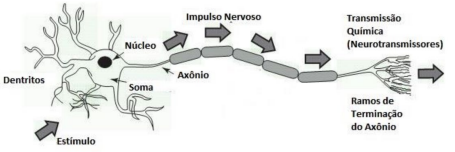
\includegraphics[width=12cm]{Figuras/celula-neural.png}
    \caption*{Fonte: \cite{rocha2022analise}}
    \label{fig:celula_neural}
\end{figure}

\section{Sistemas Sensíveis a Contexto}
Sistemas Sensíveis a Contexto são sistemas que utilizam de pistas contextuais para adaptar-se a alguma necessidade de elementos em seu ambiente. Essas pistas contextuais podem ser dados de ambiente, variáveis dinâmicas que mudam ao executar do programa ou qualquer tipo de informação que seja útil para definir características e comportamentos num cenário \cite{vieira2009modelos}. No âmbito deste projeto, o contexto ao qual o sistema será sensível é a externalização emocional do jogador, que influenciará como o próprio jogo age e reage em seu ambiente.

\section{Loop de biofeedback}
No contexto de medicina, para citar o trabalho do Dr. Michael G. McKEE na área de terapia, 
\textit{"O biofeedback envolve o monitoramento e uso de informações fisiológicas para ensinar os pacientes a modificar funções fisiológicas específicas"}\cite{biofeedback2008biofeedback}. No contexto do nosso projeto, o biofeedback participa de um círculo de interpretação e comportamento. Através dos sinais do jogador, o jogo irá adaptar-se e mudar o modo com que interage com o jogador. Com isso, o jogador tem a oportunidade de tentar controlar esses sinais afim de aproveitar melhor de um aspecto ou outro de uma mecânica. 

\section{Computação Afetiva}
Com o uso massivo de bases de dados e experimentos com o uso de inteligencias artificiais para uma interação mais humana. O termo Computação Afetiva explora justamente o comportamento das interações Humano-computador, ou seja, o modo como as maquinas podem reconhecer, interpretar e influenciar um sentimento humano. Em relação a área de jogos, o artigo \cite{filipa2019emovere} mostra a possibilidade de criar o desenvolvimento de estratégias afim de experiencias mais envolventes e personalizadas para cada jogador, onde o jogo responda ao estado emocional atual do jogador, adaptando historia, recompensas e mecânicas para determinada parte do jogo, deixando a experiência mais imersiva e satisfatória.

\break
\section{Emoções por Nível de Excitação e Valência}

 \begin{figure}[h]
    \centering
    \caption{Diagrama de Emoção por nível de Excitação e Valência}
    \centering
    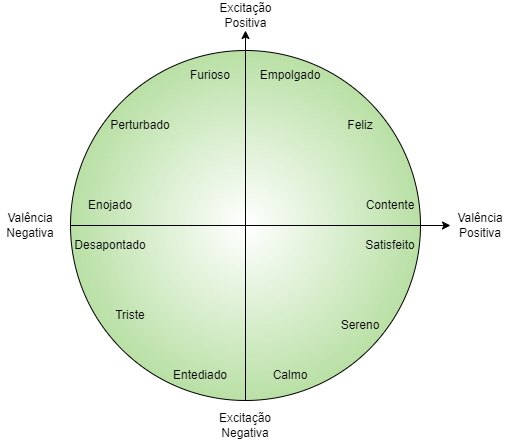
\includegraphics[width=0.5\textwidth]{Figuras/diagrama-emocional.drawio.png}
    \caption*{Fonte: Autores}
    \label{fig:diagrama_emocional}
\end{figure}

Utilizando aparelhos de medição de atividade tanto neurológica quanto fisiológica, é possível medir o nível de estresse, nervosismo ou ansiedade de uma pessoa. Cruzando esses dados com os obtidos através de uma entrevista de feedback, é possível dizer em qual direção estava apontado seu vetor emocional dentro do diagrama de excitação-valência.


    \chapter{Trabalhos Relacionados} \label{trabs}

Tendo em vista como propósito principal deste estudo a classificação em emoções de determinados sinais neurológicos e sua utilização no contexto de jogos digitais, os trabalhos \cite{nalepa2019emotionalcontext} e \cite{filipa2019emovere} foram definidos como principais modelos de estudo.

No trabalho \cite{nalepa2019emotionalcontext}, há a exploração de sistemas capazes de detectar e interpretar os sinais capturados através de equipamentos sensoriais. Foram utilizados nesse trabalho equipamentos de medição sensorial, como o kit BITalino (r)evolution \cite{bitalinoprosuto}, plataforma com diversos sensores de bio-sinais pré-montada, a Pulseira Empatica E4 \cite{empatica4site}, que é um monitor de atividade vestível, capaz de medir diversos dados fisiológicos com precisão, e outros equipamentos para efeito de comparação, como a Microsoft Band 2 \cite{Microsoftband2}, atualmente descontinuado.

Além destes materiais, foram utilizados frameworks para construção de aplicativos de teste, como o AWARE \cite{awaresite}, que é uma plataforma e plugin Android para captura de dados sensoriais, o HeaRTDroid \cite{heartdroidsite}, uma ferramenta para captura de informação contextual dinâmica e interpretação desses dados em meio a ruídos e incertezas, o BandReader \cite{bandreader}, um software que se comunica através de bluetooth com múltiplos dispositivos de aquisição de dados, bem como foram construídos protótipos de jogos afetivos feitos nas game engines Unity e GameMaker.

Para construir o ambiente de teste que, neste caso, é o jogo, foram seguidas técnicas de e Game Design Patterns, que visam definir relações e interações entre diferentes conceitos e elementos dentro de um jogo.

Este trabalho conclui-se trazendo como resultados a avaliação dos jogadores sobre quais protótipos de jogos geraram maior satisfação no que se diz sobre imersão, mecânicas e ajustes dos níveis e fases: os jogos que utilizaram Loop Afetivo ou que não utilizaram.

No trabalho \cite{filipa2019emovere}, o foco principal foi a utilização de um loop de feedback emocional dentro de uma mecânica de combate no jogo Emovere. Através de um sensor de batimentos cardíacos, o pulso do jogador seria detectado, influenciando na jogabilidade, como demonstrado no diagrama de biofeedback abaixo.

\begin{figure}[h]
    \centering
    \caption{Diagramas de loop de combate e biofeedback.}
    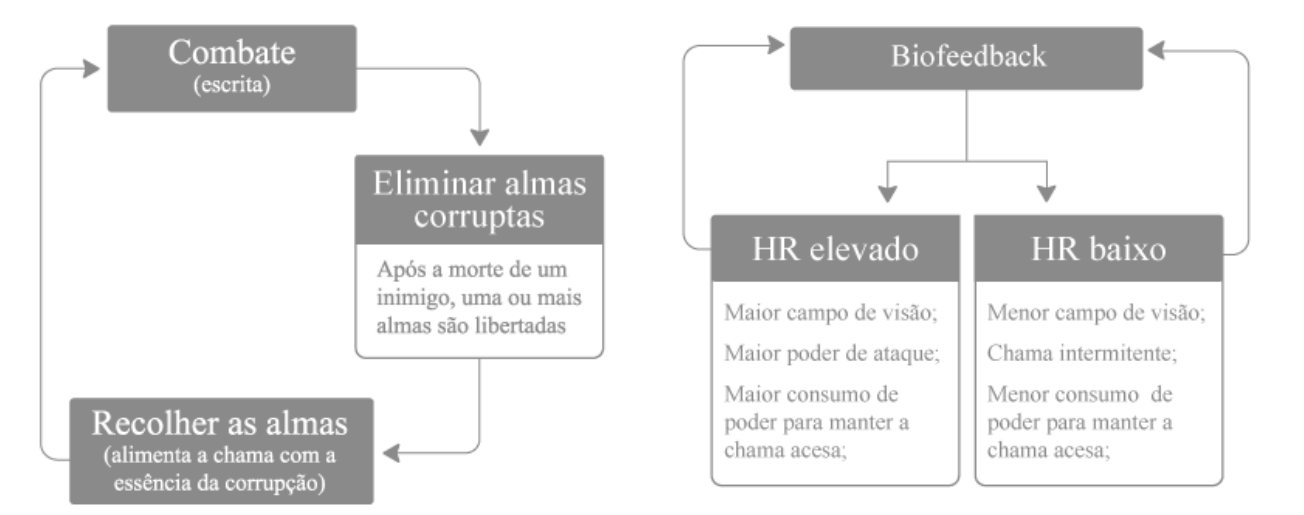
\includegraphics[width=17cm]{Figuras/diagrama-filipa-loop.png}
    \caption*{Fonte: \cite{filipa2019emovere}}
    \label{fig:diagrama_biofeedback}
\end{figure}

Os trabalhos apresentados conseguem cobrir com clareza os aspectos técnicos da implementação, através de métodos e materiais conhecidos e replicáveis. Buscamos aplicar alguns destes conhecimentos neste projeto, sendo eles a game engine Unity e o loop de biofeedback entre jogador e jogo.

Nota-se que grande parte dos recursos e conceitos extraídos e analisados nos trabalhos acima não serão utilizados neste trabalho. Isso se deve ao fato de que, na metodologia que será abordada aqui, não será utilizada detecção em tempo real. Isso está melhor descrito em \ref{metodologia}.

Além destes conteúdos, utilizamos metodologias para leituras de arquivos com dados de sinais neurais e sinais fisiológicos, técnicas de game development e integração de sistemas para agregar o jogo a um sistema de interpretação. Esses processos também estão detalhados em \ref{metodologia} 

Serão focados neste trabalho tentativas para expandir o que foi abordado nos dois projetos mencionados: enquanto ambos trabalham apenas com sinais fisiológicos, serão trabalhados entradas de sinais neurais reconhecidos.
    \chapter{METODOLOGIA}
\label{metodologia}

Será mostrado neste capitulo os materiais, ferramentas e métodos utilizados na realização deste trabalho. Em detalhes, são explicados a constituição e captação dos bancos de sinais neurais, métodos de processamento por injeção de banco de dados no algoritmo, o jogo utilizado como exemplo e as métricas utilizadas para avaliar o trabalho. \todo{listar todo o conteúdo deste capitulo quando o trabalho for finalizado}

\section{Materiais}

\subsection{Banco de Sinais Neurais e Fisiológicos}
Para esse trabalho utilizamos dados que contemplem, de alguma forma, o estado emocional de pessoas dentro de um contexto. Esses dados podem ser encontrados, nas metodologias investigadas na forma de sinais eletromagnéticos "crus" vindo de regiões conhecidas e pré estabelecidas do cérebro.

Uma das formas menos invasivas e melhor desenvolvidas para captação desses sinais é o Eletroencefalograma (EEG). Esse método consiste na utilização de eletrodos para captação de pulsos eletro-magnéticos do cérebro em determinadas regiões que, a depender do tipo de estimulo e feedback verbal do estado emocional reportado por um participante no momento da coleta, serão classificados como positivos ou negativos.

No caso deste trabalho, foram utilizados os bancos \cite{linkbase1} e \cite{linkbase2} que contem dados captados das formas mencionadas para treinar um algoritmo de reconhecimento de padrões. \todo{detalhar melhor os pormenores dos bancos}

\section{Métodos}

% Foram pensadas em duas metodologias levemente distintas em relação a captação dos dados e em como serão utilizados.

% \subsection{Detecção e Feedback Simultâneos}
% A primeira, chamado "Método com detecção e feedback simultâneos" parte do principio que a detecção dos dados, ou seja, a captação dos sinais neurais, ocorrerá ao mesmo tempo que a interpretação e utilização desses dados dentro do jogo. Este é um cenário ideal onde o loop de feedback é fluidamente realizado: o jogador, ao jogar o jogo, gera sinais que, ao serem interpretados pelo algoritmo fazem com que o jogo se adapte passivamente a esses sinais. Com isso, o jogador reage a essa adaptação, gerando um novo fluxo de sinais, e assim sucessivamente. Essa metodologia, além de depender de todos os equipamentos e programas para captação e interpretação correta de sinais, é também um grande desafio de performance e paralelismo.

% \begin{figure}[h]
%     \centering
%     \caption{Diagrama de Metodologia Paralela}
%     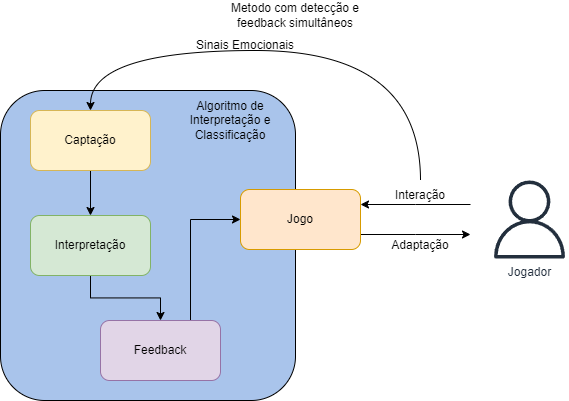
\includegraphics[width=10cm]{Figuras/diagrama-metodologia-um.drawio.png}
%     \caption*{Fonte: Autores}
%     \label{fig:diagrama_metodologia}
% \end{figure}

\subsection{Injeção de Banco de Dados}
Este método é levemente simplificado no setor de pré-interpretação com relação a uma leitura ao-vivo utilizando equipamentos de sensores EEG. Ao invés de ser utilizada a captação ao mesmo tempo que a interpretação dos dados, foi utilizado um banco de dados já classificado e conhecido. Esses dados foram injetados em um algoritmo treinado para sua interpretação e imediata utilização pelo jogo. Dessa forma, ao invés de estarmos testando a verdadeira saída emocional do jogador, focamos na capacidade do algoritmo de interpretação e do jogo de agirem ao mesmo tempo através da injeção dos dados de uma base conhecida no algoritmo. \todo{detalhar melhor o que tem na base de dados}

\begin{figure}[h]
    \centering
    \caption{Diagrama de Metodologia Classificada}
    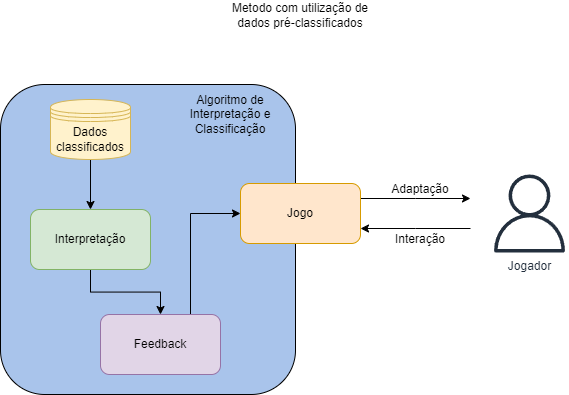
\includegraphics[width=10cm]{Figuras/diagrama-metodologia-dois.drawio.png}
    \caption*{Fonte: Autores}
    \label{fig:diagrama_metodologia}
\end{figure}

Foi optado por essa metodologia por conta da necessidade de permissões para utilizar um método que realizasse a leitura através de equipamentos de EEG durante a execução do jogo em voluntários, mas também para que o foco do trabalho seja a adaptabilidade de um sistema - nesse caso, o jogo - quando utilizada essa entrada de dados. \todo{rever a parte sobre o foco deste trabalho, a depender do desenrolar do projeto}

\subsection{Jogo}
O jogo que utilizamos como base é uma versão modificada dos projetos realizados durante as aulas de Desenvolvimento de Jogos Digitais no sétimo ciclo do curso. Se trata de um jogo de plataforma no estilo de clássicos como \textit{Castlevania} \cite{castlevania} e \textit{Super Metroid} \cite{supermetroid}, melhor detalhado a frente.

\todo{descrição do jogo do projeto. não é versão final.}
No jogo deste projeto, o jogador controla um personagem capaz de se transformar a depender da emoção do jogador. Ao se transformar, as mecânicas do jogo se alteram, mudando como o jogador deve jogar o jogo e as reações do mundo do jogo ao personagem.

O jogo passou por adaptações de compatibilidade com o algoritmo de classificação em tempo real que será desenvolvido, tanto para receber os dados como para implementar as diferentes mecânicas adaptativas.

O jogador pode jogar e testar as novas funcionalidades, por meio de inputs programáveis que serão disponibilizados no jogo. Esses inputs, através de botões, simularão a inserção da emoção do jogador, pois não é permitido captar diretamente as ondas transmitidas pelo usuário.

\section{Métricas}

Como métrica, após o teste das duas diferentes versões do jogo: com sistema de adaptabilidade e sem sistema de adaptabilidade, foi realizado um questionário com perguntas a cerca da satisfação dos jogadores comparando as duas versões. As perguntas giram em torno de três aspectos: 

\begin{itemize}
  \item Satisfação com as Mecânicas: o quanto a mudança de mecânicas agrada com relação as mecânicas padrões não-adaptativas do jogo;
  \item Satisfação com a Imersão: o quanto o jogador se sente mais imerso com relação a imersão sentida na versão não-adaptativa do jogo;
  \item Satisfação Geral: o quanto o jogador gosta mais ou menos do jogo com o sistema adaptativo com relação ao jogo sem o sistema.
\end{itemize}

Essas perguntas foram respondidas em uma escala de -5 a 5, onde -5 é muito menos e +5 é muito mais.

Além disso, foram avaliados o desempenho de algoritmos de leitura de bancos de dados com sinais neurais e fisiológicos, com relação ao tempo de execução, leitura e saída dos dados, para descobrir a viabilidade de sua utilização em simultâneo à execução do jogo. \todo{como será feito?}


    
    % \input{Texto/experimentos}
    \chapter{RESULTADOS ESPERADOS} \label{resultados}

%Baseando-se na metologia proposta e no conteúdo apresentado nos capítulos \ref{trabs} e \ref{conceitos}, este trabalho tem a pretenção de obter um sistema preditivo com boa qualidade quando comparado com outros trabalhos apresentados.

%Primeiramente, espera-se uma melhoria na precisão das predições e uma diminuição no custo computacional para gerá-las utilizando-se os modelos baseados em clusterização propostos por este trabalho em comparação com filtros colaborativos tradicionais.

%Em seguida, espera-se que o sistema híbrido proposto atinja uma precisão melhor do que a obtida por outros trabalhos que possuem sistemas também baseados em clusterização.

%Por fim, este trabalho visa comparar os resultados obtidos pelo sistema proposto com os resultados de trabalhos que utilizam outras técnicas tanto no âmbito de precisão das predições como em custo computacional para construção do modelo e para geração de predições.

Levando-se em conta o que foi observado na metodologia proposta deste trabalho, é esperado que seja obtido um modo de clusterização, onde a precisão dos filtros colaborativos supere o desempenho das técnicas encontradas atualmente.

Com isso, os sistemas de distribuição que utilizarem essas técnicas aplicadas à sua base de dados conseguirão realizar melhores predições, pois os dados em questão estarão relacionados de forma a aumentar a eficiência do sistema.
Além disso, a melhora no desempenho computacional permitirá menores custos monetários com hardware ou melhores resultados mantendo-se os mesmos recursos computacionais.

Pela observação dos aspectos analisados, esse trabalho melhorará a utilização de sistemas de recomendação. Consequentemente, trazendo benefícios aos usuários e às empresas responsáveis por esses sistemas.
    \label{conclusao}
\section{Discussão e Conclusão}


Essa parte é só para o TCC2. Essa parte é só para o TCC2 Essa parte é só para o TCC2Essa parte é só para o TCC2Essa parte é só para o TCC2Essa parte é só para o TCC2Essa parte é só para o TCC2Essa parte é só para o TCC2Essa parte é só para o TCC2Essa parte é só para o TCC2Essa parte é só para o TCC2Essa parte é só para o TCC2Essa parte é só para o TCC2Essa parte é só para o TCC2


Essa parte é só para o TCC2. Essa parte é só para o TCC2 Essa parte é só para o TCC2Essa parte é só para o TCC2Essa parte é só para o TCC2Essa parte é só para o TCC2Essa parte é só para o TCC2Essa parte é só para o TCC2Essa parte é só para o TCC2Essa parte é só para o TCC2Essa parte é só para o TCC2Essa parte é só para o TCC2Essa parte é só para o TCC2Essa parte é só para o TCC2


Essa parte é só para o TCC2. Essa parte é só para o TCC2 Essa parte é só para o TCC2Essa parte é só para o TCC2Essa parte é só para o TCC2Essa parte é só para o TCC2Essa parte é só para o TCC2Essa parte é só para o TCC2Essa parte é só para o TCC2Essa parte é só para o TCC2Essa parte é só para o TCC2Essa parte é só para o TCC2Essa parte é só para o TCC2Essa parte é só para o TCC2


Essa parte é só para o TCC2. Essa parte é só para o TCC2 Essa parte é só para o TCC2Essa parte é só para o TCC2Essa parte é só para o TCC2Essa parte é só para o TCC2Essa parte é só para o TCC2Essa parte é só para o TCC2Essa parte é só para o TCC2Essa parte é só para o TCC2Essa parte é só para o TCC2Essa parte é só para o TCC2Essa parte é só para o TCC2Essa parte é só para o TCC2


Essa parte é só para o TCC2. Essa parte é só para o TCC2 Essa parte é só para o TCC2Essa parte é só para o TCC2Essa parte é só para o TCC2Essa parte é só para o TCC2Essa parte é só para o TCC2Essa parte é só para o TCC2Essa parte é só para o TCC2Essa parte é só para o TCC2Essa parte é só para o TCC2Essa parte é só para o TCC2Essa parte é só para o TCC2Essa parte é só para o TCC2


    
}

\printbibliography

%\printindex

\end{document}